\section{Related Works}%
\label{sec:related_works}
%
\subsection{Geometric control for trajectory generation}
%
Operational space control was the first control method that imposed
a desired dynamical system onto a robotic system \cite{Khatib1985,Khatib1987}.
The concept was an important step toward naturally controlling 
kinematically redundant robots. The concept was formalized in the field 
of geometric control, where the study of differential geometry leads to 
stable and converging behavior under geometric conditions \cite{bullo2019geometric}.
More recently, RMPs for manipulation tasks offered
a highly reactive trajectory generation method \cite{Ratliff2018,Cheng2020}. This method
achieves composable behavior by introducing a split between the importance metric
and the forcing term. Using the \textit{pullback} and \textit{pushforward} operator
to change between manifolds of the configuration space, individual 
components, such as collision avoidance and goal attraction, can be designed
iteratively. However, RMPs require intuition and 
experience when being designed, and convergence 
can only be proven conditionally \cite{Ratliff2020}. Later, optimization fabrics
were introduced that are able to completely decouple importance metrics
and the defining geometry. Under simple construction rules for these 
two components, convergence can be easily guaranteed \cite{Ratliff2020,Xie2021,Li2021,meng2019neural}.
In our prior work on optimization fabrics, the framework was first applied to
mobile manipulation and generalized to more dynamic environments. \cite{Spahn2023}.
%
\begin{figure}[t]
    \centering
    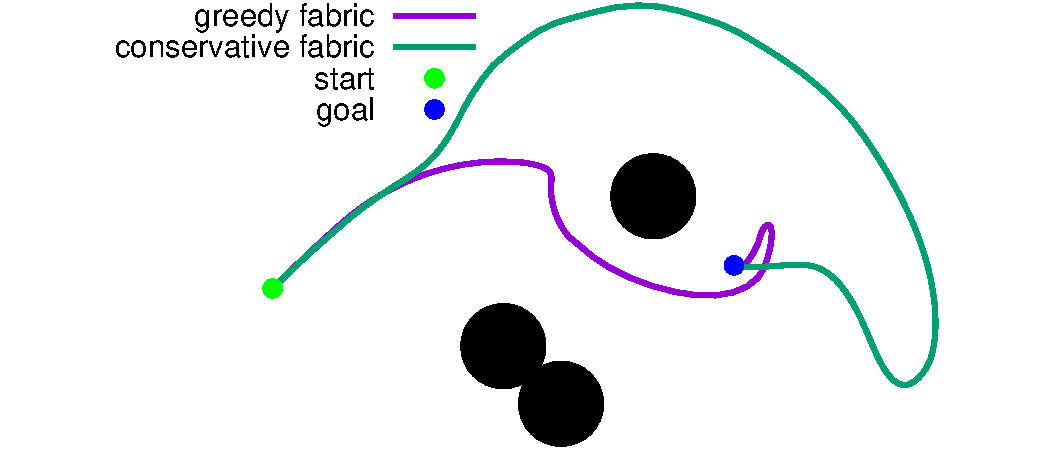
\includegraphics[width=0.8\linewidth]{effect_tuning}
    \captionsetup{belowskip=-10pt}
    \caption{Two different parameter sets for optimization fabrics given the same problem. While the greedy tuning
    is more aggressive (purple), the more conservative tuning results in a smoother trajectory (green).}
    \label{fig:effect_tuning}
\end{figure}
%

\subsection{Autotuning for trajectory generation}
%
Autotuning can be beneficial for trajectory generation when using model predictive control.
In \cite{loquercio_autotune_2022}, an autotuned
model predictive controller has outperformed a manual tuned controller of the same kind by 
25\%. Jointly optimizing parameters and the model of the controller, \textit{AutoMPC} 
showed the benefit of parameter tuning in the context of simultaneous system
identification and control \cite{edwards_automatic_2021}. These methods are explicitly 
formulated for model predictive control and do not transfer easily to other trajectory generation
methods. In contrast, we propose a generic parameter optimization approach to trajectory generation.

\subsection{Hyperparameter tuning in machine learning}
%
Within the machine-learning field, hyperparameter tuning has shown to be highly 
important for all different kinds of applications \cite{yang2020hyperparameter,hutter_automated_2019,optuna}. 
Parameter optimization aims to minimize 
training costs while achieving the best possible performance. Hyperparameter tuning 
is most valuable in extremely
costly applications such as reinforcement learning \cite{zoph_neural_2017}. Generally, two different search
algorithms have been investigated: grid search and random search \cite{bergstra_random_nodate}.
Current state-of-the-art methods for parameter search are based on 
random search with a Bayesian optimizer \cite{optuna,bergstra_algorithms_nodate}.
While the machine-learning community has largely agreed on the importance of
parameter tuning, systematic tuning of trajectory generation methods are not well established. 
In this paper, we showcase, with the example of optimization fabrics, how important 
parameter tuning is and how trajectory generation can benefit from it.
